
\chapter{Connected Cars} \label{CARS}
\smallskip
\hfill
\begin{minipage}[b]{8cm}
%{\it This work was presented in part at the conference of one-legged deaf-mutes in Quiberon in April 1994.}
\end{minipage}
%\begin{flushright} Remoi \end{flushright}
\vskip 2cm


\section {The software revolution}
\medskip
{\Huge E}mbedded software is one of the key innovation in the automotive world. From the paper of
 Robert Charette (\cite{Cha2009}) published in IEEE Spectrum, the first car embedding a software was the Oldsmobile Toronado from General Motors in 1977. The Toronado enclosed an \gls{ecu}\@ which managed the spark timing. In 1978, General Motors offered on the Cadillac Seville as an option a trip computer able to display the speed, the fuel level, trip and engine information. This product was based on an embedded version of a Motorola 6802 and had about 50,000 lines of code. Since, more and more functions are performed by software in a car. To limit the volume of cable in a car, all the sensors and on-board unit are now connected to a network backbone using CAN or xxx network. As the computing power of the processor grows, new functions appear in cars. Cars become now on-wheel software platform like airplanes or trains.A modern family car embeds between 30 and 50 ECUs performing the management of the multiple systems(see \ref{tab:soft}). A premium car can have up to 3,000 singular functions performed by software.   

\FloatBarrier
\begin{table}
\centering
\begin{tabular}{| l | l | l |}
\hline
Airbag & ABS & Anti-thief system \\
\hline
Air Conditioning & Speed control & motor management \\
\hline
Turn signals & Headlights & Klaxon \\
\hline
Seat management & Navigation system & Audio system\\
\hline
Wheel pressure & management of the doors and windows & ... \\
\hline
\end{tabular}
\caption{Software function in a car}
\label{tab:soft}
\end{table}
\FloatBarrier


In 2009, Alfred Katzenbach, Director of Information Technology Management at Daimler announced that the radio and navigation management system of an S-class Mercedes-Benz contains over 20 millions line of code and the car embeds nearly as many ECUs as an Airbus A380 (excluding the in-flight entertainment system) (\cite{Cha2009}). Software in a car has an exponential growth in size and complexity. In just 10 years, the software volume in a car expands by a factor 10, to arrive at around 150 million of lines of code. A model S from Tesla is equipped with a 17' tactical display based on a Linux kernel which controls almost every driver functions. In fact, there is only 2 manual buttons that are not management by software in the car, the blinker and the glove's compartment.


A side effect of this revolution is the complexity and the richness of the functions proposed to the driver. It is frequent to have the driver manual of a car with over 500 pages to explain all the driver functions. Automotive experts estimate that an average driver uses not more than 20\% of those functions. Thus is why, some automotive manufacturers are asking them the question of a limitation (or reduction) of software functions proposed in a car. For example, is it really necessary to have the ceiling light of a car going out gradually when the doors are closing?\\

The growth of the software in a car has also important consequences on the way to maintain and repair a car. An estimation gives that more than 50\% of the ECU that are changed by a car mechanic have no software or hardware failure. Mechanic frequently replaces pieces without the knowledge of the root cause of the issue. Now, one of the most frequent activity of a car mechanic is to download and upgrade new version of software. Some car manufacturer, like Tesla proposes to download software updates, including software corrections (patches) or new functionalities, using the cellular network without any involvement of a car mechanic.


Today, the cost of the software and the supporting electronic in a car is estimated between 35\% and 40\% of the cost of a car. Investment to develop new software platform became so expensive that the main European Automotive manufacturers develop a series of standards to reduce the developent cost:
\begin{itemize}
    \item a commom platform; \emph{Automotive Open System Architecture (AUTOSAR)} \cite{AUTOSAR} allowing there suppliers to develop a single platform interoperable between several manufacturers. 
    \item a software development framework for the safety; \emph{Road vehicles, Functional Safety package} ISO 26262 \cite{ISO26262}
    \item and recently a standard to address the cybersecurity management system; \emph{Road vehicles - Cybersecurity engineering} ISO 21434 \cite{ISO21434}.
\end{itemize}

Introduction of software in the car permits to have safer and less polluting cars but it has open the door at two new risks the \emph{software safety risk} and the \emph{cyber-security threat}. 

\section {Modern car software architecture}

\subsection {AUTOSAR}

\gls{autosar}\@ was founded in 2003, with the goal to develop an architecture, independent of the underlying ECU hardware that the automotive industry can use to reduce the increasing complexity of software in modern vehicles (\cite{AUTOSAR}). This is the de facto standard for the automotive software today. AUTOSAR makes an abstract layer of the underlying hardware, so that the applications written on top of AUTOSAR are independent from the actual supplier of the ECU hardware. The AUTOSAR standard documentation guides companies and the automotive industry in designing and implementing software in their vehicles. Besides the Software architecture and the Standardized \gls{api}\@, AUTOSAR provides a Software development methodology. By adopting the AUTOSAR standard, companies can develop software solutions that are independent of the hardware they are running on, and this software can run on any ECU in the vehicle. 
\bigskip

AUTOSAR is a three-layered architecture (\cite{AUTOSAR_archi}): 
\begin{itemize}
    \item the \emph{application layer} provided by the software company implementing the specific functions of the ECU. This is the highest layer which contains the software components (SWCs). AUTOSAR application (e.g., ABS, Cruise Control $\ldots$) consists of several SWCs, which provide the core functions. An AUTOSAR SWC is an atomic piece of software that cannot be divided and is located a single ECU. 
    \item the \emph{run-time environment (RTE) layer}. The RTE layer provides the standardized interface between the SWCs and the basic software layer. Because of this layer, SWCs can be used on different ECUs, independent of the ECU vendor.
    \item the \emph{basic software (BSW) layer} that consists of four sub-layers; the \emph{services layer} providing operating system functions like communication services, memory services, diagnostic services, $\ldots$. The layer also contains the main security mechanisms. The \emph{ECU abstraction layer} makes higher software layers independent of ECU hardware layout. It provides an application programming interface to devices regardless of their location (internal/external of the microcontroller). The \emph{Microcontroller abstraction layer}. It contains drivers for direct access to the upderlying microcontroller and internal parameters. It makes higher layers independent of the microcontroller. The \emph{complex drivers layer} which provides the ability to integrate special-purpose functions such as drivers for devices that are not specified with the AUTOSAR standard. This layer accesses directly the microcontroller. 
\end{itemize}

Each of the sublayers offers different services as shown in \ref{fig:AUTOSAR_archi}. 

\FloatBarrier
\begin{figure}
    \includegraphics[width=\textwidth]{AUTOSAR_architecture}
    \caption{AUTOSAR layered architecture}
    \label{fig:AUTOSAR_archi}
\end{figure}
\FloatBarrier

The AUTOSAR standard defines security mechanisms that can be used by the software modules implemented into the vehicle system. It further specifies interfaces and procedures to provide Secure On-Board Communication, and the exact implementation is left for the OEMs to decide on. OEMs choose the cryptographic algorithms and encryption techniques which they want to implement and use in the vehicle system.


AUTOSAR has been mainly build to ensure a high level of Safety of the system. Many safety mitigations requested by the standard can be attack vectors. For example (see \cite{Nas2017}), to protect the internal and external communication, AUTOSAR defines the \Gls{ete}\@ library which defines the safety mitigations to prevent safety critical functions from operating on faulty or missing data. The mitigations are:
\begin{itemize}
    \item \Gls{crc} check to detect corruption of data
    \item Sequence counter to detect out of sequence messages and to osrt the messages
    \item Alive counter to prevent operating on old data
    \item A unique ID for Interaction Layer Protocol Data Unit (I-PDU) group to detect a fault of sending I-PDU on unintended message
    \item Timeout monitoring to detect communication loss with the sender.
\end{itemize}

Attack based on those mitigations will lead to a rejection of the messages and a potential \Gls{dos}\@. No mechanism has been provided to detect the difference betwwen a non-malicious errors in the content of a message and an attack.




\subsection {The software stacks}

\begin{tbd}
Commencer a pr\'esenter les diff\'erentes couches logiciel.\\

The following four stacks could become the basis for upcoming generations of cars in five to ten years:
\begin{itemize}

\item \emph{Time-driven stack}. In this domain, the controller is directly connected to a sensor or actuator while the systems have to support hard real-time requirements and low latency times; resource scheduling is time based. This stack includes systems that reach the highest Automotive Safety Integrity Level classes, such as the classical Automotive Open System Architecture (AUTOSAR) domain.
\item \emph{Event- and time-driven stack}. This hybrid stack combines high-performance safety applications, for example, by supporting ADAS and HAD capability. Applications and peripherals are separated by the operating system, while applications are scheduled on a time base. Inside an application, scheduling of resources can be based on time or priority. The operating environment ensures that safety-critical applications run on isolated containers with clear separation from other applications within the car. A current example is adaptive AUTOSAR.
\item \emph{Event-driven stack}. This stack centers on the infotainment system, which is not safety critical. The applications are clearly separated from the peripherals, and resources are scheduled using best-effort or event-based scheduling. The stack contains visible and highly used functions that allow the user to interact with the vehicle, such as Android, Automotive Grade Linux, GENIVI, and QNX.
\item \emph{Cloud-based (off-board) stack}. The final stack covers and coordinates access to car data and functions from outside the car. The stack is responsible for communication, as well as safety and security checks of applications (authentication), and it establishes a defined car interface, including remote diagnostics.
\end{itemize}

\url{https://www.mckinsey.com/industries/automotive-and-assembly/our-insights/rethinking-car-software-and-electronics-architecture}
\end{tbd}


\FloatBarrier
\begin{figure}
    \includegraphics[width=\textwidth]{architecture}
    \caption{Architecture g\'en\'erique}
    \label{fig:archi}
\end{figure}
\url{https://www2.deloitte.com/us/en/insights/focus/future-of-mobility/pure-play-software-in-automotive-industry.html}
\FloatBarrier

Bla bla bla


\section {Le risque cybers\'ecurit\'e pour l'automobile}
 \medskip
 {\Huge L}'ajout de logiciels et de connectivit\'e....


3 niveaux d'attaques:
\begin{itemize}
\setlength\itemsep{1em}
\item \emph{Attaques physiques}. 
\begin{itemize}
\item Attaque via la prise diagnostique de la voiture. L'objectif est de pouvoir modifier les caract\'eristiques de la voiture et/ou de rajouter des options sur la voiture. Les logiciels d'une voiture sont hautement configurables. Un m\^eme logiciel est install\'e sur plusieurs gammes de v\'ehicules d'un constructeur. La diff\'erenciation entre les deux mod\`eles s'effectue par le param\'trage du logiciel. Si un attaquant \`a la possibilit\'e de modifier ces param\`etres, il peut activer des fonctions optionnelles de la voiture ou modifier les caract\'eristiques moteur pour booster le v\'ehicule.
\item Attaque via la prise USB de la voiture. L'objectif est de pouvoir cr\'eer un point d'entr\'ee pour une attaque courte ou longue port'ee sur le v\'ehicule. La prise USB peut \^etre connect\'ee sur un \'equipement radio qui permet d'\'etendre la port\'ee de l'attaque.
\end{itemize}

\item \emph{Attaque courte port\'ee} L'objectif est de pouvoir prendre le contr\^ole du v\'ehicule, d'envoyer de fausses informations ou de bloquer les communicatiosn aux v\'ehilcules aux alentours. De plus en plus de voitures ont un syst\`eme d'ouverture de portes et de d\'emarrage sans cl\'e.Par exemple, votre voiture est gar\'ee devant votre maison et les cl\'es sont sur le petit d'entr\'ee.  Un attaquqant peut ins\'erer un \'equipement radio entre la cl\'e et la voiture (attaque par relais). Un c\^ot\'e est proche de la voiture, lautre c\^ot\'e est connect\'e \`a une antenne scannant les fr\'equences radio de la cl\'e. Ceci permet d'ouvrir et/ou de d'emarrer la voiture m\^eme quand les cl\'es du v\'ehicule sont hors de port\'ee de la voiture. Une fois que l'antenne a accroch\'e la fr\'equence de la cl\'e, elle relaye son signal sur l'\'equipement proche du v\'ehicule. La voiture a ainsi l'impression que le propri\'etaire est proche et ouvre les portes et autorise la d\'emarrage. Le v\'ehicule peut \^etre vol\'e sans effraction (voir \url{https://www.youtube.com/watch?v=_cua7BFX-Qk} pour un video d'attaque relais). Un autre exemple, consiste \`a brouiller le signal pour la fermeture centralis\'ee d'un v\'ehicule. Le conducteur appuie sur le bouton de fermeture centralis\'ee de sa cl\'e, il a le sentiment que sa voiture est correctement ferm\'ee. Mais si le signal est brouill\'e, la voiture est ouverte et un attaquant peut facilement ouvrir un porte pour voler des affaires dans la voiture.
 
\item \emph{Attaque longue port\'ee}. L'objectif est de prendre le contr\^ole \`a distance d'un v\'ehicule. Un des fameux exemple de ce type d'attaque est la prise de contr\^ole d'une Jeep Cherokee par 2 attaquants; Andy Greenberg conduisait sa voiture sur l'autoroute vers Saint-Louis, roulant \` 70 mph. 2 hackers Charlie Miller et Chris Valasek sont install\'es dans leur canap\'e avec leur laptop ouvert. Dans un premier temps, la climatisation de la voiture s'est affol'ee, puis, une image des 2 hackers est apparue sur l'\'ecran de la voiture, la radio a chang\'e de station et le volume a fortement augment\'e, Mr Greenberg ne pouvait pas contr\^oler le volume de la radio ni la station. Ensuite la voiture s'est arr\^et\'ee toute seule. (voir \cite{Mil2015} pour le d\'etail de l'attaque)
\end{itemize}



\section {Car architecture over time }

\begin{figure}[h]
    \centering
	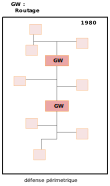
\includegraphics[width=0.45\textwidth]{schema/architecture/1980.pdf}
    \caption{Architecture 1980}
    \label{1980_archi}
\end{figure}

\begin{figure}[h]
    \centering
	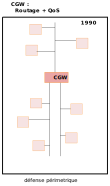
\includegraphics[width=0.45\textwidth]{schema/architecture/1990.pdf}
    \caption{Architecture 1990}
    \label{1990_archi}
\end{figure}

\begin{figure}[h]
    \centering
	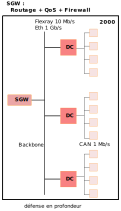
\includegraphics[width=0.45\textwidth]{schema/architecture/2000.pdf}
    \caption{Architecture 2000}
    \label{2000_archi}
\end{figure}

\begin{figure}[h]
    \centering
	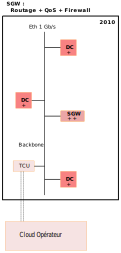
\includegraphics[width=0.45\textwidth]{schema/architecture/2010.pdf}
    \caption{Architecture 2010}
    \label{2010_archi}
\end{figure}

\begin{figure}[h]
    \centering
	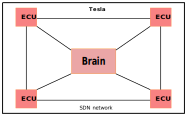
\includegraphics[width=0.6\textwidth]{schema/architecture/tesla.pdf}
    \caption{Architecture tesla}
    \label{tesla_archi}
\end{figure}



\section {Car Architecture we used}

\begin{sidewaysfigure}[h]
    \centering
	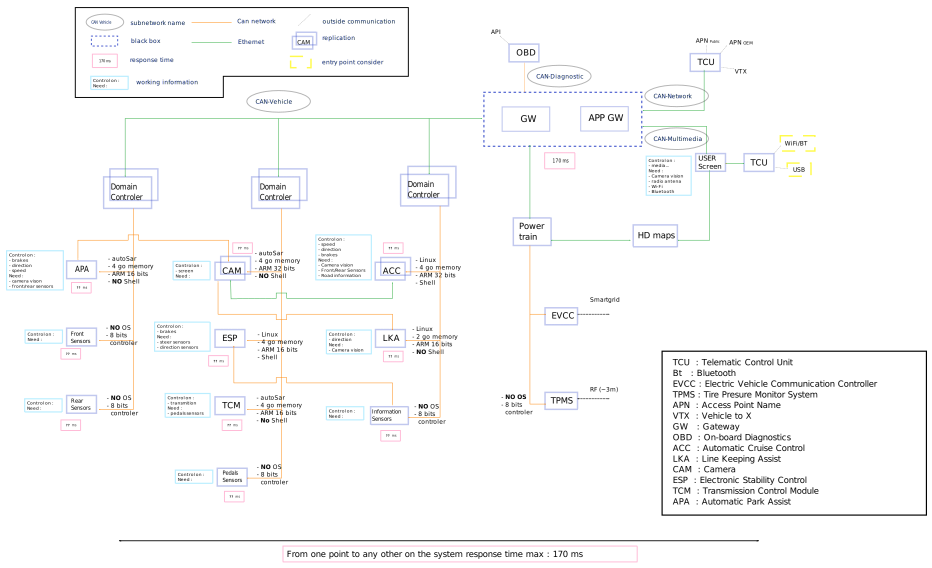
\includegraphics[width=1\textwidth]{schema/architecture/Car_complete_architecture.pdf}
    \caption{The architecture we used}
    \label{used_archi}
\end{sidewaysfigure}




\section {Existing Attacks}

\section {Existing Defense}
